\documentclass[10pt,a4paper,oneside]{article}

\usepackage[swedish]{babel}
\usepackage[utf8]{inputenc}
\usepackage[T1]{fontenc}
\usepackage{graphicx}
\usepackage{color}
\usepackage{url}
\usepackage{hyperref}
\usepackage[nomarkers]{endfloat}

\renewcommand{\efloatseparator}{\mbox{}} 
 
\title{GoodMarket}
\author{Erica Eriksson, Johanna Sörbom, Malin Torestam}
\date{\today}

\begin{document}

\maketitle
\newpage

\section{Sammanfattning}
I denna rapport presenteras en affärsmodell för Goodmarket. Detta är en nätbaserad tjänst som främjar försäljning av närproducerade produkter. GoodMarket vill förenkla för småskaliga producenter i Stockholmsområdet att konkurrera med importerade varor från butiker och nå ut till fler miljömedvetna kunder. Detta är en tjänst som ligger i tiden och fyller ett växande behov i ett samhälle där miljö- och klimattänk blir allt vanligare. I denna rapport diskuteras affärsmodellens hållbarhet i olika framtidsscenarion och alternativa utvecklingar av modellen för att klara av att konkurrera på dagens marknad. I den riktning samhället är på väg mot förväntas denna affärside ha en bra chans att växa sig stark. Hur detta ska gå till kommer att diskuteras i denna rapport tillsammans med svagheter och förbättringsmöjligheter. 
\newpage

\tableofcontents
\newpage

\section{Introduktion}
I dagens globaliserade samhälle står transport av varor för en stor del av de miljöfarliga utsläppen som negativt påverkar vårt klimat. En stor del av de varor vi konsumerar dagligen fraktas långa sträckor fram och tillbaka mellan länder innan de hamnar i butiken. Idag kommer t.ex hälften av all den mat vi lägger på tallriken från andra länder. Genom att välja lokalt producerade varor kan denna energikonsumtion minskas dramatiskt \cite{Naturskyddsföreningen2}. För att uppnå ett hållbart samhälle och en hållbar konsumtion av varor krävs att vi jobbar tillsammans för att öka kvaliteten och minska utsläppen av de varor vi konsumerar. GoodMarkets syfte är att förenkla för småskaliga producenter i Stockholmsområdet att konkurrera med importerade varor från butiker och nå ut till en större kundkrets. Genom att välja närproducerat minskas miljöpåverkan på klimatet samtidigt som tillverkningsprocessen kan övervakas och påverkas för hälsosammare, miljövänligare alternativ. 

\newpage

\section{Bakgrund}
Mat är en stor del av vår vardag, Matproduktion och transport av mat är en otroligt stor bov till klimatförändringarna idag. Folk i Sverige äter 45 procent mer kött nu till skillnad mot 90-talet, men denna siffra börjar allt mer stanna av på grund av den allt mer vegetariska trenden som växer fram \cite{Naturskyddsföreningen1}. Men trots detta färdas mycket av den mat vi äter långa sträckor över hela jorden. Samtidigt har maten aldrig varit så billig som nu. En helt ny marknad har växt sig fram runt matkulturen, idag finns det färdigkomponerade matkassar som kommer fram ända till ens bostad allt för att handlingen ska gå snabbt och vara bekväm. Butiker ökar även sitt sortiment av ekologiska varor för att möta efterfrågan hos konsumenter \cite{ICA2}. För några år sedan användes knappt begreppet EKO och idag är nästintill varenda vara märkt med detta. Men dessa ekologiska varor har ofta transporteras långa vägar över jordklotet. För att både bli mer hälsosamma samt minska klimatpåverkan från råvaror krävs stora livsstilsförändringar \cite{Jordbruksverket}. \\
 
I jakten på att odla så mycket råvaror som möjligt på kort tid och liten yta så har det lett till att råvarorna som främst är grönsaker och frukt har blivit näringsfattiga. De innehåller därmed inte den mängd näringsämnen som de gjorde förr vilket gör att man måste äta mer av dessa varor för att uppnå sitt dagliga behov. Viktiga antioxidanter som exempelvis lykopen finns i betydligt lägre halt på odlade grödor jämför med grödor som tar mer plats \cite{SR}. Studier visar att ekologiska grödor innehåller mer antioxidanter än vanligt odlade grödor pga att de inte blir besprutade med bekämpningsmedlen eller kväve. Det leder till att grödorna själva behöver producera mer fytokemikalier för att överleva och dessa fytokemikalier är viktiga antioxidanter för människan. Dock är det är väldigt svårt för konsumenter idag som söker efter bra och näringsrika råvaror, för att finna det behöver man ofta åka till en marknad eller komma i kontakt med bönderna själv.\\
 
Matkulturen är som allt annat en trend som kommer och går och påverkas av samhället i stort. De senaste åren har allt fler människor börjat bry sig om sin hälsa genom att både träna bra men även få i sig bra näring. Denna trend har lett till att konsumenter vill ha bra råvaror som är närodlade, inte är fulla av bekämpningsmedel och är bra för miljön. Folk är idag villiga att betala lite mer för att få i sig bra mat och samtidigt ha ett gott samvete om att maten är bra med rättvisa produktionsvillkor, liten miljöpåverkan och att skötseln av djur är bra (branschinfo). Även fler och fler övergår till att minska mängden av kött de äter och blir därmed flexitarianer, eftersom kött står för stora delen av utsläppen av växthusgaser. Detta leder till att de behövs bra råvaror som har hög näringstäthet för att folk fortfarande ska få i sig tillräckligt med näringsämnen. Men att hitta närodlade råvaror i storstäder är inte enkelt. Det finns många småskaliga bönder men det är både svårt för dessa att nå ut till konsumenterna samtidigt som det är krångligt, bökigt och tar tid för konsumenterna att finna dessa varor. Därför finns ett behov av en tjänst som på ett enkelt sätt kopplar ihop dessa småskaliga bönder med intresserade konsumenter.\\
 
Trots alla sociala medier är det idag svårt för småskaliga bönder att nå ut till en stor kundkrets och det är vad en tjänst som kopplar ihop konsumenter med bönder lösa. En annan trend i dagens samhälle är att allting ska vara så enkelt och bekvämt som möjligt. Folk är inte villiga att behöva lägga sin tid på något som exempelvis handling av mat utan istället väljer de att betala en extra summa och få till och med färdigkomponerade matkassar hem till dörren. Denna trend gör det ännu svårare för småskaliga bönder att nå ut till sina kunder eftersom folk inte har varken tiden eller intresset att finna bra råvaror.\\

I en tid där det är de stora köpcentrumen eller internetsidorna som lockar är det svårt för små egenföretagare att synas och nå ut till potentiella kunder. Dessa företagare har ofta genuina, vackra och bra produkter men har kanske lite svårt med sin marknadsföring, både för att det är dyrt och tidskrävande. Därför är det svårt för nya företag att etablera sig på marknaden, det behövs tjänster som hjälper dessa små företag att både nå fler kunder men också att växa.\\
 
På grund av detta behov har GoodMarket skapats. En enkel tjänst för konsumenter att handla närodlade råvaror och genuina produkter,  men även ett enkelt sätt för jordbrukare, bönder och egenföretagare att öka sina kundkrets och försäljning. I denna tjänst når konsumenter småföretagare som tillverkar produkter med känsla och bra villkor. Det ska vara enkelt att hitta information och varor samt att handla. Detta kan jämföras med färdiga matkassar som antingen hämtas i butik eller körs hem till kunden \cite{ICA2}. Detta är ett fenomen som blivit större och större i Sverige med fler och fler företag erbjuder denna tjänst. Denna tjänst gör det enkelt för konsumenter att kunna få näringsrika och bra producerade råvaror samt genuina produkter direkt hem till dörren. 

\newpage

\section{Metod}
Denna rapport grundar sig på litteraturstudier samt en marknadsundersökning som skickats ut till 51 st småskaliga bönder i stockholmsområdet. Marknadsundersökningen hittas under Figurer längst bak i rapporten.
\newpage

\section{Beskrivning av tjänsten}
\subsection{Vad erbjuder vi för tjänst?}
Denna tjänst är en e-handel som binder samman småskaliga producenter av främst livsmedel men även skönhetsprodukter, accessoarer och dylikt med konsumenter som är intresserade av hälsosamt och miljövänligt producerade produkter. Denna tjänst erbjuder ett sätt för småskaliga producenter att marknadsföra sina produkter och öka sin försäljning. Tjänsten ska alltså fungera som en marknadsplats som binder samman producenter med konsumenter. För konsumenterna erbjuds ett enkelt sätt att handla närproducerade produkter av bra kvalitet. Det innebär livsmedel som produceras av småskaliga bönder, såsom ägg, olika grönsaker, kött, mejeriprodukter, fisk från småskaliga fiskare samt även vissa förädlade varor såsom ost och sylt. Utöver detta avses skönhetsprodukter såsom tvålar och bodylotion samt smycken, kläder, fårskinnsfällar, möbler och nära tillverkade köksverktyg m.m. Ytterligare en möjlighet är viltkött från jaktlag som har överskott och önskar sälja detta. 

För företag samt privatpersoner kommer det att erbjudas färdiga ihopplockade säsongsanpassade korgar som passar som presenter till familjen eller kollegorna. Dessa kan t.ex innehålla choklad, frukt och en bodylotion.  

\subsection{Hur blir man medlem?}
När den här tjänsten är ny på marknaden kommer producenter att aktivt rekryteras till tjänsten. Dessa kommer att besökas och upplysas om fördelarna med att använda denna tjänst och erbjudas medlemskap. När tjänsten sedan är en aning mer välkänd ska nya producenter själva ha möjlighet att ansöka om att gå med via hemsidan. När nya gårdar och producenter ska läggas till i tjänsten kommer dessa att besökas för att dels kontrolleras att de når upp till de standarder som krävs och dels för att ta bilder på produkter och livsmedel som ska säljas. Detta är för att det ska finnas professionella bilder på hemsidan så att det ser snyggt ut för konsumenter. Dessa bilder kommer att läggas till i ett konto för den specifika producenten. Sedan är idén att producenten själv kontinuerligt ska kunna uppdatera mängden varor som finns för försäljning på respektive profil.  

\subsection{Vad krävs för att bli medlem?}
För att få vara representerad på denna hemsida ska man uppfylla vissa krav. Dessa krav ska säkerställa för konsumenter att de produkter som inhandlas förhåller sig till tjänstens värderingar angående miljövänlighet och hälsa. Vissa krav ställs däremot av logistiska skäl. Några exempel på krav är:  

\begin{itemize}
\item Verksamheten ska ligga inom Stockholms län, med vissa undantag. 
\item Krav gällande odling och bekämpningsmedel.
\item Krav för hur djur behandlas. 
\item KRAV-märkning krävs ej men det uppmuntras.  
\item Minimigräns för produceringsmängd. 
\item Registrerat företag.
\item Uppfyller EU-direktiv och lagar kring försäljning för sina produkter.
\end{itemize}

Exakt vilka krav som ska ställas måste utvärderas ytterligare innan tjänsten lanseras för att säkerställa att betydelsefulla lagar och riktlinjer för olika typer av produkter följs på korrekt sätt. Dessa krav kommer därefter kontinuerligt att kontrolleras för alla producenter som representeras på hemsidan. 

\subsection{Hur ska hemsidan och appen utformas?}
Varje producent kommer att ha en egen hemsida med information om dess verksamhet och de produkter de säljer. Det kommer att finnas möjlighet att filtrera sökningar på både producenter och på produkter. Tjänsten ska sedan fungera som en e-handel där man lägger sina produkter i varukorgen och betalar online. Information om leverans kommer att meddelas när kunden har lagt produkter i varukorgen och bestämt leveranssätt. Hemsidan kommer även att ha en FAQ sida samt kontaktuppgifter till en kundtjänst. Hemsidan kommer att ha bilder samt information om alla producenter/gårdar och produkter som representeras för att ge konsumenterna en känsla för var produkterna kommer ifrån. Medlemskap för konsumenter kommer att vara valfritt och gratis men om man blir medlem så kommer man att ha en egen profil där man kan se vad man har beställt och följa produktens leverans. Det kommer även att gå att få förslag på produkter som passar en själv utifrån vad man tidigare har beställt. Medlemmar har även möjligheten att lägga en återkommande order, t.ex. varje vecka. En app som är lätt att använda kommer även att utformas så att man lätt kan lägga beställningar och följa sin order via mobilen.  


\subsection{Kvalitetskontroll}
I tjänsten kommer det att finnas ett betygssystem, vilket innebär att konsumenter som köper varor från en specifik producent kan betygsätta kvalitén på dessa varor och lämna kommentarer. Detta betyg samt kommentarerna kommer vara synliga för andra konsumenter som är intresserade av att handla från samma producent. På detta sätt kan kvalitén på varorna kontrolleras kontinuerligt och konsumenterna kan känna sig säkrare på att det är bra varor de handlar om andra användare har lämnat bra betyg. GoodMarket kommer även kontinuerligt att utföra kvalitetskontroller hos producentmedlemmar för att upprätthålla bra standard och se att de krav som finns för producenterna upprätthålls. 

\subsection{Förpackning av varor}
GoodMarket tillhandahåller en tjänst för försäljning av produkter som kommer att marknadsföras som hemtrevlig och möjligen lite exklusivare. Att vara billigast på marknaden är inte målet, istället erbjuds varor som är bättre för miljön och kunden. Därför kommer producenterna att ha möjlighet att köpa förpackningar via tjänsten om de inte har egna som de vill använda. Dessa förpackningar kommer att vara glasflaskor och papperskassar. På detta sätt minskas förbrukningen av engångsförpackning och produkten ser mer exklusiv ut. För presentkorgarna och företagskorgarna används korgar i ett bra val av material. Om konsumenten handlar kontinuerligt kan korgarna tas tillbaka av GoodMarket och sedan återanvändas. 

\subsection{Order och leverans}
Orden läggs på hemsidan eller i appen och beställningen levereras på torsdagar och söndagar. Dessa dagar har valts för att de troligtvis är mest gynnsamma för konsumenter. Leverans på torsdag ger varor till helgen och leverans på söndag ger varor inför vardagarna. Detta kommer att kräva en viss framförhållning från kundens sida. Olika leveransalternativ kommer att finnas möjliga för kunden, hemleverans eller upphämtning på GoodMarkets lager. Priserna beror på vilket alternativ kunden väljer. Leverans i Stockholms innerstad sker via cykelbud för att minska miljöpåverkan vilket är en viktig del i GoodMarkets arbete. Transporten från producenter samt till kunder utanför innerstaden kommer att skötas med egen miljövänlig transport av GoodMarket för att kunna säkerställa miljövänlig leverans. 
\newpage

\section{Koppling till energisystemet}

Syftet med denna tjänst är att främja konsumtion av närproducerade, miljövänliga produkter.  I dagens globaliserade samhälle där den ökande konsumtionen av importerade varor står för en stor del av utsläppen av växthusgaser är närproducerade varor ett viktigt steg i utvecklingen mot ett hållbart samhälle \cite{Naturskyddsföreningen1}. Genom att främja närproducerat kan vi minska transportkostnader på miljön i form av utsläpp och öka Sveriges möjligheter att överse och påverka produktionsprocessen. Att flytta produktionen till Sverige minskar inte bara utsläppen från transport utan ökar även transparensen i framställningen av produkten. Att transportera en vara från t.ex Spanien släpper ut betydligt mer koldioxid än transport av samma vara från en producent i Stockholm. \\  

Vi jämför utsläppen från transport av en vara, exempelvis tomater, från Nynäshamn till Sveavägen i Stockholm jämfört med tomater från Barcelona. För att beräkna detta används utsläppsberäknaren My Climate \cite{MyClimate}. Att transportera varor med en dieselbil som drar 6l L per 100 km från Nynäshamn till Sveavägen i Stockholm släpper ut 0.016 ton koldioxid. Att istället frakta varor från Barcelona till Arlanda med flyg och sedan köra dem till en butik på Sveavägen släpper ut 0.01 ut från bilentransporten och 0.46 ton ut för vikten av en person under flygresan. Detta blir 0.47 ton totalt. Detta är en ungefärlig uppskattning, endast transport har tagits i åtanke och även där har förenklingar gjorts. Transporten av tomaterna från odling i Spanien till Barcelonas flygplats har försummats. Inte heller vikt av tomaterna har tagits i åtanke vid transporten i bil. Detta ger inte en exakt uppskattning med det är tillräckligt för att dra slutsatsen att det sker betydligt mindre utsläpp från transport vid frakt från Nynäshamn jämfört med import från Spanien. Beräkningen behandlar inte heller att GoodMarket i största mån avser använda elbil för transport vilket skulle öka skillnaden i växthusgasutsläpp ytterligare vid jämförelse av de båda alternativen.

\newpage

\section{Canvas modellen}
I detta avsnitt presenteras hur affärsmodellen för GoodMarket läggs upp enligt Business Model Canvas. Affärsmodellen för en tjänst som denna kan se ut på många olika sätt, och det finns flera tillvägagångssätt samt olika kombinationer av tillvägagångssätt. Därför diskuteras olika scenarion för alternativa affärsmodeller i avsnitt 11.2. 

\subsection{Värdeerbjudande}
Denna tjänst erbjuder ett sätt för småskaliga producenter att marknadsföra sina produkter och öka sin försäljning. Tjänsten ska fungera som en marknadsplats som binder samman producenter med konsumenter. För konsumenterna erbjuds ett enkelt sätt att handla närproducerade produkter av bra kvalitet. \\

En del av värdeerbjudandet handlar om att göra närproducerade produkter mer lättillgängligt för konsumenter. Konsumenterna får enklare åtkomst till närproducerade produkter, medan producenterna får bättre tillgång till potentiella kunder. Samtidigt spelar bekvämligheten också en stor roll för värdeerbjudandet. Användarna kan enkelt hitta information om de produkter som erbjuds från varje producent och kan sedan bekvämt lägga en beställning via hemsidan eller app. Denna tjänst är värdedriven och strävar inte efter att vara billigast på marknaden utan istället erbjuda bra kvalité och miljövänlighet på ett enkelt sätt.  


\subsection{Kundsegment}
Denna tjänst riktar in sig till småskaliga producenter i Stockholmsområdet. Dessa kommer huvudsakligen att bestå av småskaliga bönder som säljer ägg, grönsaker, kött och mejeriprodukter. Men även småskaliga fiskare och förädlade varor såsom ost och sylt är välkomna. Utöver detta säljs även skönhetsprodukter såsom tvålar och bodylotion samt smycken, kläder, fårskinsfällar, möbler och närtillverkade köksverktyg. Ytterligare möjlighet är också viltkött från jaktlag som har överskott och önskar sälja detta. \\

En del av kundsegmentet är även de konsumenter som köper produkterna via hemsidan. Dessa kommer att vara medel- och höginkomsttagare som har ett intresse för hälsosamma, miljövänliga, närproducerade produkter. Företag som använder sig av exempelvis fruktkorgar och presenter till sina anställda är ytterligare ett kundsegment. 

\subsection{Kanaler}
Denna del av affärsmodellen ska beskriva hur olika kundsegment får information om värdeerbjudandet samt hur värdeerbjudandet ska levereras till det kundsegmentet. Det handlar även om hur kunder ska kunna återkoppla och få hjälp med tjänsten som erbjuds. Det finns flera olika kundsegment och dessa kräver olika kanaler. Det kommer att finnas en hemsida och en mobilapplikation som är själva plattformen där producenter och konsumenter kopplas ihop. Det är först och främst via denna hemsida som medvetenhet om tjänsten skapas hos de olika kundsegmenten. Ytterligare marknadsföring kommer att ske främst genom sociala medier som Facebook och Instagram, men även genom så kallade ambassadörer. Detta är inflytelserika personer i samhället som provar tjänsten och sprider budskapet om den vidare genom olika kanaler. \\

Ett annat mål för marknadsföring är att få med tjänsten på jämförelsesidor, vilket skulle vara ytterligare ett sätt att öka medvetenheten bland konsumenter om att denna tjänst finns. Ett alternativ är webbsidan hittamatkassen.se som är gratis att finnas med på. Där det går att jämföra matkassar baserat på flera olika parametrar. Det går bland annat att leta efter ekologiska matkassar \cite{Hittamatkassen}. GoodMarket skulle kunna användas som en matkasse och kan därför platsa på en jämförelsesida för sådana. Denna marknadsföring riktar sig till alla kundsegmenten, men kanske främst till konsumenterna då en annan typ av kundrelation kommer att finnas gentemot producenterna. Se avsnitt 7.4. \\

För konsumenterna kommer den viktigaste kanalen vara hemsidan och appen. Genom dessa köper de sina varor från de olika producenterna som finns med i tjänsten. På hemsidan och i appen kommer kunderna också kunna få svar på enklare frågor gällande tjänsten via en FAQ-sida, eller få mer hjälp genom att hitta kontaktinformation till personer som kan svara på fler frågor. Konsumenterna kommer också att kunna utvärdera produkter med hjälp av betygssystemet på hemsidan och i appen och genom det hjälpa till att säkerställa tjänstens kvaliteté. Detta ger också producenterna en möjlighet att få återkoppling från sina kunder. \\ 

Leverans av de varor som konsumenterna köper via  hemsidan eller appen kommer att ske på olika sätt beroende på kundens önskan. Kunden kommer alltså att kunna välja olika leveransalternativ vid själva köpet. Om kunden väljer leverans till dörren kommer kunden behöva betala den fraktkostnaden, men det är viktigt att detta alternativ ändå är en möjlighet även om det kostar mer. Självklar ska ett alternativ också vara att hämta varorna själv på GoodMarkets lager. Transporten kommer att skötas med egen miljövänlig transport av GoodMarket för att kunna säkerställa miljövänlig leverans. I innerstan kommer cykelbud att leverera varorna till kunden och vid leverans längre ut kommer transporten ske med miljövänligt utkörning av GoodMarket.\\

Producenterna kommer också att använda sig av hemsidan och appen till stor del. Genom denna uppdaterar de lagersaldot på varor så att konsumenterna vet vad de kan köpa. De marknadsför sig också via hemsidan genom bilder och information om gården eller vad som än är kopplat till det som de producerar. 


\subsection{Kundrelation}
Kundrelationer kommer att skilja sig beroende på vilket kundsegment som betraktas. För producenterna kommer denna relation även att variera över tid. I början kommer dessa producenter, dvs. småskaliga bönder eller företagare i Stockholmsområdet, eller mindre fiskare eller osttillverkare m.m. att aktivt rekryterats till tjänsten genom hembesök där värdeerbjudandet pitchas för var och en. Detta är för att bygga upp en kundkrets så att tjänsten kan lanseras. När producenterna ansluter sig till tjänsten måste deras produkter/varor/gårdar kontrolleras så att de håller vissa standarder. Även detta kommer att ske via hembesök och utförs med jämna mellanrum. I samband med den första kvalitetskontrollen kommer också de varor som producenten önskar sälja via tjänsten att fotograferas så att det finns professionella bilder på hemsidan. Detta blir alltså en mycket personlig relation med producenterna till att börja med. Allt eftersom tjänsten blir vanligare så kommer denna relation bli en aning mer automatiserad då producenterna inte behöver rekryteras aktivt utan kan istället ansöka att gå med i tjänsten direkt via hemsidan. \\

För konsumenterna är relationen till största del automatiserad via hemsidan. Om konsumenterna väljer att bli medlemmar i tjänsten kommer de att ha ett eget konto där de kan se vad de har handlat förut. De kommer även att få förslag på rekommenderade varor baserat på vad de har köpt tidigare. De kan även hjälpa varandra via hemsidan genom att betygsätta varor som de handlat, det blir alltså en typ av forum för alla användare. Där användarna kan hjälpa varandra hitta kvalitativa produkter. 


\subsection{Intäktsström}
Intäkterna kommer att bestå av en månadskostnad samt en procentuell avgift på vinsten från försäljningen. Genom att dela upp intäkterna från två olika källor kan företagets inkomst bli stabilare och mer säker. Månadskostnaden kommer att säkerställa en grundinkomst som täcker en del av det allra viktigaste för företaget. Utöver detta kommer en procentuell avgift på 10 procent av vinsten att tas av företaget. Denna procent är baserad på marknadsundersökning, se bilaga X. Detta är en osäker inkomstkälla som beror på mängden sålda varor. Däremot kan det kännas bra för producenterna som vet att GoodMarket måste leverera och har i sitt eget bästa intresse att öka försäljningen av deras produkter för att få in en stadig inkomst. För de kunder som inte har egna förpackningar kommer det erbjudas möjlighet till att köpa det av GoodMarket. Detta kommer främst att vara en tjänst till kunderna men innebära en liten inkomst. Utöver detta kommer ett reklamblad att följa med i leveranserna där producenterna själva eller andra företag kan köpa annonsplats vilket då skapar ytterligare en intäktsström. Slutligen kommer också en intäkt genereras från försäljningen av de färdiga presentkorgarna som levereras. \\

Möjligheter till bidrag från KTH Innovation finns för att starta upp affärsmodellen. Det finns även bidrag att få från EU \cite{EU}. Företaget “Gårdsbudet” som har en liknande affärside men endas handlar med livsmedel har nyligen fått ett innovationsstöd från europeiska jordbruksfonden för landsbygdsutveckling \cite{Gårdsbudet4}. Detta är något som även GoodMarket hoppas kunna få stöd från.  

\subsection{Nyckelresurser}
Nyckelresurserna består av flera olika typer av resurser. De fysiska nyckelresurserna är främst fordon för leverans och upphämtning av produkter. Det krävs cyklar som ska användas för transport i innerstaden. Då denna transport är en nyckelaktivitet som kommer att outsourcas kommer dessa resurser från en nyckelpartner. Lastbil eller skåpbil för ytterligare transport är däremot en egenägd fysisk resurs som kommer behövas. Mänskliga resurser kommer att krävas i form av anställda som utför dagligt arbete för att tjänsten ska fungera, det vill säga chaufför. Även anställda programmerare som förbättrar och underhåller tjänsten behövs. Samarbeten med olika nyckelpartners är intellektuella resurser som kommer behövas. Detta omfattar samarbete med cykelbudfirma, leverantör av miljövänliga förpackningar och papperskassar, och med viktiga aktörer för marknadsföring av tjänsten.  Slutligen är också hemsidan och appen nyckelresurser som är ytterst viktiga för att kunna leverera tjänstens värdeerbjudande. 

\subsection{Nyckelaktiviteter}
En nyckelaktivitet kommer vara att hämta varor hos producenter och sedan leverera dessa på ett bra sätt till konsumenter. Detta är troligtvis den aktivitet som kommer utföras oftast och är därför viktigt att det fungerar på ett bra sätt, speciellt då mycket av kundrelationerna kommer att påverkas av denna aktivitet. Marknadsföring spelar också stor roll kundrelationer och är en annan nyckelaktivitet. I denna aktivitet ingår att upprätthålla relationer med aktörer inom tjänstens marknadsföring, det vill säga de ambassadörer som används samt ansvariga för marknadsföring inom sociala medier. Det ingår även att utveckla de reklamannonser för tjänsten som är tänkt att spridas via sociala medier. Innan tjänsten är väletablerad i samhället är även en nyckelaktivitet att aktivt rekrytera producenter till tjänsten för att bygga upp en kundbas.\\  

Andra nyckelaktiviteter handlar om underhåll av tjänsten för att den ska fungera på ett bra sätt och leverera det värdeerbjudande som beskrivs. Det innebär att plattformen, det vill säga hemsidan och appen, måste uppdateras och förbättras regelbundet för att följa med i utvecklingen. De producenter som är kopplade till tjänsten måste också kvalitetskontrolleras regelbundet för att stämma av att de följer de standarder som tjänsten kräver. När det kommer till producenter kommer också en nyckelaktivitet vara att granska nya producenter som önskar gå med i tjänsten samt att hjälpa till med att fotografera bilder till hemsidan. 

\subsection{Nyckelpartners}
Cykelbudfirma och leverantör av miljövänliga förpackningar är nyckelpartners som används för att förhoppningsvis optimera den andel nyckelaktiviteter samt nyckelresurser som finns inom företaget. Även ekonomin förbättras troligtvis genom att använda dessa nyckelpartners då mängdrabatt är möjligt för dessa tjänster och varor. Aktörer inom marknadsföring är också en nyckelpartner som används för att öka medvetenheten om tjänsten hos potentiella kunder. Det syftar då främst på de ambassadörer som kommer användas. 

\subsection{Kostnadsstruktur}
Denna tjänst kommer att vara värdedriven vilket innebär att för att driva tjänsten kommer en del aktiviteter ha ett högre pris än det billigast möjliga priset. Ett exempel är leverans som kommer att ske delvis med cyckelbud som vanligtvis har ett högre pris än andra bud. Detta för att miljövänlighet spelar en stor roll i tjänstens värdeerbjudande och därför anses tjänsten vara värdedriven.\\ 

Kostnadsstrukturen består delvis av vissa startkostnader som krävs för att få tjänsten att fungera. Till dessa kostnader hör bil, kylskåp och inredning, hårdvara för programutveckling samt ursprunglig utveckling av plattformarna som tjänsten verkar på. Dessa kommer att betalas av i takt med att företaget växer och blir mer lönsamt. Det kommer även att finnas en del löpande kostnader. Dessa kommer initialt försöka täckas av inkomsterna från försäljningen. Till dessa hör löner till anställda, transport av varor, program för webbutveckling, marknadsföring samt hyra av lokal.  


\newpage

\section{Marknadsundersökning}
I den marknadsundersökning som skickades ut till småskaliga producenter av livsmedel i Stockholmsområdet framkom att 64.3 procent inte tror att kunden känner till dem när de ska köpa varor. Utöver detta framgick att 78.6 procent är intresserade av att nå ut till fler privatpersoner och 64.3 procent är intresserade av att använda den tjänst som GoodMarket erbjuder. En 10-20 procent avgift på vinsten är det populäraste alternativet som dessa kunder valt medans en månadsavgift på 150-200 kr också ses som ett möjligt alternativ för kunderna. Majoriteten av kunderna har svarat att det inte behöver hjälp med förpackningar till sina varor medans 28.7 procent har svarat att de vill ha det. Detta kan då ses som ett alternativ för de som vill använda sig av denna tjänst. Svarsmängden på denna marknadsundersökning har varit låg och dessa siffror baseras en låg mängd svar. Se bilaga X för detaljer. 

\newpage

\section{Ekonomisk budget}
För att GoodMarket ska gå runt krävs 3 anställda. En chef som sköter ekonomi och kundrelationer, en programutvecklare som sköter hemsidan och appen samt en som sköter leveranser och förpackning av varor. Cykelbud kommer att outsourcas och förpackningar kommer att köpas in. \\

Vi har utgått från antagandet att varje konsument handlar för 500 kr/gång exklusive moms. GoodMarket tar 10 procent av denna vinst, dvs. 50 kr per köp. Om vi antar att vi i början har 20 producenter som vardera betalar en månadsavgift på 99 kr behöver vi få in 1 166 765 kr i inkomst från procenten av vinsten. Detta betyder att en omsättning på 1 190 525 kr/år behövs för att täcka de löpande utgifterna. För att detta ska vara möjligt behövs 23 336 st betalande kunder per år, dvs 1945 st betalande kunder i månaden. Detta visas i scenario 1 som är det fall som vi valt att utgå ifrån. I detta fall täcks endast de löpande kostnaderna och ej engångs kostnaderna. \\

Fraktkostnaden kommer att täckas av kunden. Då cykelbud används kommer detta att bli något dyrare än andra leveransalternativ men det antas att ett bra avtal kan fås vid regelbunden användning av tjänsten \cite{Movebybike}. I denna budget försummats försäkring till bilen och drivmedel. \\

I tabellen nedan refereras till 3 scenarier. Scenario 1 är fallet då inkomsterna precis täcker de löpande utgifterna. Detta sker då vi representerar 20 producenter och säljer till 1945 st kunder för 500 kr varje månad. Scenario 2 är fallet då tjänsten går bra och antalet kunder, dvs inkomsterna överstiger utgifterna. I detta fall räknar vi med att representera 40 producenter och ha 4000 betalande kunder per månad. Scenario 3 är fallet då vi ännu inte har tillräckligt många kunder för att täcka de löpande utgifterna, vi representerar endast 10 producenter och har 100 st betalande kunder per månad. 

\newpage

\section{Konkurrenter}
Det finns ett företag i Sverige som heter Gårdsnära som driver en hemsida som heter gardsnara.se. Denna hemsida tillhandahåller en söktjänst för att hitta närproducerad mat och dryck och tjänsten finns även som mobilapplikation till iPhone och iPad. Deras vision är att skapa en relation mellan producenter och konsumenter i hela Sverige, för att genom det underlätta handel mellan dem \cite{Gårdsnära2}, \cite{Gårdsnära3}. Söktjänsten innehåller 1991 registrerade producenter vilket gör dem till Sveriges största söktjänst för närproducerade livsmedel \cite{Gårdsnära4}. Det är gratis för företag att registrera sig på Gårdsnära, men det går att köpa till en tilläggstjäns som ger bättre annonsering för 160 kr/månaden \cite{Gårdsnära5}. De har också vissa kriterier för vilka företag som får gå med \cite{Gårdsnära1}. Det går däremot inte att handla varor via Gårdsnära och de uppger också på sin hemsida att de inte har möjlighet att granska alla producenter samt hålla informationen om de uppdaterad \cite{Gårdsnära2}.\\

Den största skillnaden mellan GoodMarket och Gårdsnära kommer självklart vara att det går att handla varor via GoodMarket men inte via Gårdsnära. Detta kommer göra att värdeerbjudandet för GoodMarket, när det gäller konsumenterna, kommer innehålla mer enkelhet och bekvämlighet eftersom konsumenterna slipper att själva kontakta producenterna utan handeln kan istället skötas direkt via GoodMarket. Det kommer förhoppningsvis även göra det enklare för producenterna, då de får en plattform för att både marknadsföra sig och bedriva handel. För att detta värdeerbjudande ska fungera krävs det att GoodMarket tillhandahållna tjänst kan konkurrera med antalet producenter som gårdsnära har samarbeten med. Därför är det av stor vikt att rekrytera producenter till tjänsten. Förhoppningsvis kommer tjänsten även erbjuda större värde då producenterna kommer att kvalitetskontrolleras regelbundet, medan Gårdsnära uppger att de inte har möjlighet att granska varje producent.\\

Även om de betalande kunderna är producenterna så är det också viktigt att tänka på vad konsumenterna vill få ut av denna tjänst. För att skapa ett värde med denna tjänst för producenterna krävs det att konsumenterna vill använda tjänsten. Ju fler som handlar via GoodMarket desto större värde. Därför finns det också en viss konkurrens om dessa konsumenter som måste beaktas. Vad gör egentligen att människor vill handla genom denna tjänst? En relativt stor konkurrent på detta område är vanliga matvarubutiker som säljer ekologiska produkter. Dessa produkter kan självklart konkurrera med de varor som troligtvis kommer säljas via tjänsten då de kan ses som relativt hälsosamma och miljövänliga. Därför måste tjänstens värdeerbjudande för konsumenterna erbjuda något utöver detta. Det kommer vara en  större möjlighet att se ursprunget till de varor som inhandlas. De produkter som hittas på hyllan i matvarubutiker erbjuder vanligtvis inte någon enkel möjlighet för konsumenten att förstå var produkten kommer ifrån \cite{Naturskyddsföreningen3}. Det kan också tänkas vara svårt för konsumenter att förstå vad det faktiskt innebär att produkten är ekologisk. Genom denna tjänst kan konsumenterna se exakt varifrån varorna kommer och läsa om hur produktionen ser ut, till exempel på en småskalig bondgård. Detta erbjuder en annan typ av upplevelse som ökar GoodMarkets värdeerbjudande. \\

Ett företag i USA som heter GrubMarket erbjuder en tjänst med liknande värdeerbjudande som GoodMarket och kan därför också ses som en konkurrent. De erbjuder konsumenter att köpa livsmedel från lokala bondgårdar, fiskare och certifierade privata kök. Samtidigt erbjuder de producenter en plattform för handel. De verkar dock bara i USA vilket gör att de blir geografiskt begränsade \cite{Grubmarket1}. Det gör att GoodMarket har ett övertag i Sverige och möjligtvis Sveriges grannländer. GrubMarket inriktar sig även endast på handel med livsmedel och mat \cite{Grubmarket1}. \\

Ytterligare ett liknande företag som, till skillnad från GrubMarket, verkar i Sverige är Gårdsbudet. Gårdsbudet verkar för att främja det lokala jordbruket samt att ge människor i Stockholm enkel tillgång till lokalt odlad färsk mat. Då deras hemsida, gardsbudet.se, kan man beställa både livsmedel och vissa förädlade livsmedel samt läsa om de olika gårdar som varorna kommer ifrån \cite{Gårdsbudet3}. Professionella bilder som ser relativ exklusiva ut kan ses på hemsidan för varje produkt som kan köpas. De förpackning som som syns i dessa bilder verkar endast vara producenternas egna förpackningar och inte något som Gårdsbudet tillhandahåller. I skrivande stund finns 24 olika producenter listade på hemsidan \cite{Gårdsbudet2}. Gårdsbudet levererar enligt ett leveransschema och direkt till slutkundens dörr. Vilket är det enda leveransalternativet listat under leverans i deras villkor \citep{Gårdsbudet1}. Gårdsbudets värdeerbjudande liknar GoodMarkets i och med att båda tjänsterna erbjuder en koppling mellan producenter och konsumenter. Den största skillnaden är att Gårdsbudet, till synes, endast riktar sig till bönder och småskaliga gårdar eller liknande producenter som behandlar mat och livsmedel. GoodMarkets kommer däremot att rikta sig till flera producenter, inte endast producenter av livsmedel eller liknande utan även producenter av, bland annat,  skönhetsprodukter och smycken. Detta kommer ge ett ökat kundsegmentet jämfört med Gårdsbudet vilket innebär att det finns fler möjliga producenter, som också är de betalande kunderna och bidrar med intäksström. Detta kan också tänkas skapa ett större värde för konsumenterna då de har fler produkter samlade på samma plats. Fler konsumenter ökar i sin tur intresset för ännu fler producenter att ansluta sig till tjänsten. \\

En stor del av GoodMarkets värdeerbjudande består också av en strävan efter att skapa en tjänst som främjar miljön och som främjar en beteendeförändring i samhället, när det gäller konsumtion,  som leder till ett mer hållbart samhälle. Därför är miljövänlighet viktigt och alla aktiviteter strävar efter att påverka miljön så lite som möjligt. Transporten ska planeras smart så att bil behöver användas så lite som möjligt. Det innebär att leveranser i innerstaden kommer att köras cykelbud för minska koldioxidutsläpp. Det kommer också att finnas ett alternativ för konsumenterna att hämta sina varor själva i lagerlokalen och därmed även slippa fraktkostnad. Detta är för att konsumenterna ska veta att de agerar miljövänligt genom att handla via GoodMarket samtidigt som det blir relativt enkelt. Detta skiljer sig från Gårdsbudets värdeerbjudande då de inte marknadsför någon tydlig miljövänlighet genom hela varukedjan. De påpekar däremot sin miljövänlighet i produktionssteget. 

\newpage

\section{Analyser}
Två typer av analyser kommer att presenteras. Den första handlar om olika scenarier baserat på olika sätt som tjänsten kan skötas på. Det vill säga hur olika intäktsströmmar, leveransalternativ m.m., troligtvis kommer att påverka utvecklingen av tjänsten och företaget. Den andra typen är en scenarioanalys och handlar om hur yttre faktorer kommer att påverka utvecklingen av tjänsten och dess framgång. Det vill säga olika möjliga samhällsutvecklingar skapar problem eller möjligheter för tjänsten. 

\subsection{Val av affärsmodell}
Hur intäktsströmmarna utformas kan tänkas påverka affärsmodellen i hög grad. I den presenterade affärsmodellen genereras intäkter främst från producenter som är anslutna till tjänsten. Tjänsten har då blivit ett typ av verktyg som producenterna kan använda för att sälja sina produkter och som de därför betalar för. Ett annat alternativ skulle kunna vara att intäkter tas ut från konsumenterna, det vill säga att lägga på en kostnad på priset som producenterna tar för sina varor. Tjänsten skulle då fungera som en typ av grossist som köpte in varor från olika producenter och säljer dem vidare med ett visst pålägg. För producenterna skulle tjänsten då vara en återförsäljare av deras produkter. Det skulle kunna påverka antalet kunder som använder tjänsten eftersom produkterna på det viset blir dyrare och kunder kan möjligtvis vända sig till andra liknande produkter som kan konkurrera bättre i pris. Det är alltså möjligt att det skulle innebära fler konkurrenter. Den typen av intäktsström som presenteras i affärsmodellen gör följaktligen tjänsten mer unik och gör att det fyller ett annat behov i samhället vilket kan tyckas vara mer innovativt.\\  

Ett annat viktigt val i affärsmodellen handlar om hur kanalerna utformas, närmare bestämt transport av produkter till slutkunden. Det finns ett överflöd av olika alternativ för transport som alla har både för- och nackdelar. Det enklaste alternativet är att inte ha någon transport alls utan istället endast hänvisa till att konsumenterna får hämta produkterna själva hos producenten, men det skulle underminera hela tjänstens värdeerbjudandet då enkelheten spelar en stor roll. Det skulle troligtvis också innebära mer jobb för producenterna och då denna tjänst ska fungera som ett verktyg för dem är det inte en önskvärd konsekvens. Det alternativ som har presenterats i affärsmodellen har tagits fram utifrån vad som gör tjänsten enkel för konsumenter och producenter att använda samtidigt som logistiken ska fungera effektivt. Därför sker transport endast på utsatta dagar men då är det möjligt för kunden att få leverans hela vägen fram till dörren eller så kan kunden göra valet att hämta produkterna själv i lagerlokalen i innerstaden. Detta transportsätt har även valts för att konkurrera på ett bra sätt med liknande affärsmodeller samt att det har utvecklats med en miljövänlig dimension för att komplettera värdeerbjudandet. En möjlig utveckling av kanalerna i affärsmodellen innefattar nyttjande av ombud för leverans av produkter. Om förmånliga samarbeten skulle kunna slutas med passande företag för ombud skulle det kunna vara ett utomordentligt sätt att sköta transport på ett enkelt och miljövänligt sätt då leverans inte skulle vara lika tidsberoende. Passande företag för ombud kan vara gym eftersom människor regelbundet besöker dessa vilket skapar bekvämlighet, men det skulle krävas mycket organisatoriska insatser och skulle behöva undersökas närmare innan försök genomförs. Alternativt kan ett noga urval av passande produkter levereras till gym som ombud.\\

Vilket kundsegment tjänsten riktar sig till är en annan faktor i affärsmodellen som är av stor vikt. I detta fall är Det frågan om en värdedriven tjänst vilket gör att det inte kommer vara det billigaste alternativet på marknaden vilket möjligtvis kommer göra att främst hög- eller medelinkomsttagare använder tjänsten. Därför har valet gjorts i affärsmodellen att trycka aningen extra på hemtrevlighet och exklusivitet för att inriktningen sker till det kundsegmentet. Detta är också anledningen till att professionella bilder på produkterna kommer att användas på hemsidan istället för att producenterna tar sina egna bilder.


\subsection{Scenarioanalys  - yttre faktorer}

ICA har tagit fram en rapport för hur matkulturen kommer se ut de närmsta 100 åren och hur 00-talets personer ser på mat. Där har de tagit fram olika scenarier för år 2040 som är helt olika och något av dessa kommer utvecklingen troligtvis gå åt. De kommande scenarierna baseras främst på hur matkulturen kommer se ut och inte till produkter i stort baserade på ICAs rapport 100 år och framåt \cite{ICA3}. \\ 

Farm City - Där man skapar jordbruksmark i städerna genom att bygga växthus på höjden, ha odlingar på hustak och egna hemmaodlingar. Detta scenario skulle gynna GoodMarket då det skulle finnas gott om bra och otroligt närproducerade råvaror. Samtidigt kan de ge konkurrens eftersom värdeerbjudandet GoodMarket har beror främst på att det idag är väldigt svårt att få tag i närproducerade och lokala produkter. Detta scenario är otroligt bra ur ett miljöperspektiv, då råvarorna inte behöver transporteras långt. Exempelvis kan ett höghus tillgodose dagsbehovet av grönsaker till 24 000 personer. Odling ger även bättre luft i staden, fin miljö och isolering då växtligheten är på byggnaders tak och väggar. Så då detta gynnar GoodMarket finns risken att det kommer vara så enkelt att få tag i närproducerade produkter att denna tjänst inte behövs. En utveckling av GoodMarket skulle kunna vara att GoodMarket skapar dessa kommersiella växthus i staden, samtidigt kan det dessvärre konkurrera ut småbönder på landsbygden. Så för att GoodMarkets affärsmodell ska fungera i detta scenario krävs att man går från att producenterna är småskaliga bönder på landsbygden till att de är växthus inne i staden. Då kan produkterna transporteras ut med cykelbud direkt från jordbruket och man slipper de transportsträckor som krävs idag. Det gör att produkterna kan bli billigare och de blir mindre utsläpp. \\

Mångfalldsjordbruket - I detta scenario så använder man mikroorganismer och insekter för att förbättra jordbruket och göra så näringsämnen i jorden blir enklare för grödorna att ta upp. Carbon Farming används där kolet binds i mark och växter vilket är otroligt bra för klimatet. Jordbruket har gått från att vara storskaligt och genmodifierat till att odla beroende på platsens förutsättningar, detta leder till att markerna mår bättre och kan användas mer. Samtidigt krävs inte heller lika stora mängder onaturliga medel. Man går tillbaka mot hur jordbruket var förr i tiden, med att markerna sätter gränserna. Djur som insekter används för att äta upp skadedjur, så då krävs inte farliga bekämpningsmedel.  Råvarorna blir då mer näringsrika och växter och grödor värdesätts mer då folk insett att man inte kan konsumera kött som man tidigare gjort. Kosten kommer till största delen vara växtbaserad. Detta scenario skulle gynna GoodMarkets affärsmodell då folk kommer efterfråga bra, naturliga och närproducerade produkter allt mer och det kommer även finnas fler bönder som kan möta efterfrågan. Vad som kommer krävas av GoodMarket är att de finner bra jordbrukare som producerar de mest smak- och näringsrika råvarorna. För även i detta scenario bryr sig folk otroligt mycket om sin hälsa och vill ha bra produkter. Om GoodMarkets tjänst redan är igång inom snar framtid kommer de kunna utveckla tjänsten i sådan omfattning att när detta scenario sker så har de samarbete med många producenter och även ett stor utvecklad kundnät som kommer växa allt mer då efterfrågan ökar. Tillsammans med jordbrukarna kommer ett större sortiment av växtbaserade produkter tas fram. \\

Konsumtionssamhället försvinner - I framtiden kommer folk att ha förstått att alla produkter som konsumeras har stor påverkan på klimatet och konsumtionen kommer behöva minskas för att nå miljömålen. Detta sätter press på att de produkter som konsumeras är av bra kvalite, lång hållbarhetstid och är närproducerade så de har så liten påverkan som möjligt på klimatet. Detta scenario kommer gynna GoodMarket otroligt mycket då det passar affärsmodellen, men om folk konsumerar mindre kan det självfallet märkas av även hos GoodMarket. Då krävs att de producenter för företaget väljer att samarbeta med har hög kvalité. Att marknadsföra varor med väldigt liten miljöpåverkan och med så liten råvaruåtgång som möjligt kommer vara viktigt för att tillgodose konsumenternas intressen. Att GoodMarket väljer så miljövänliga alternativ både sett till transport men även i vilka förpackningar produkterna levereras i kommer vara positivt för även sådana faktorer kan tas med när konsumenten väljer företag. 

\subsection{SWOT- analys}
En SWOT- analys på affärsmodellen är väldigt viktigt för att se vad affärsmodellen kan utvecklas. Styrkor med GoodMarkets affärsmodell är att den har ett värdeerbjudande som bygger på flera olika faktorer. Dessa faktorer är att det är miljövänligt, genuint och ger en sorts mysfaktor som ger en stor kundkrets. Att det är värdedrivet kan anses som positivt utifrån konsumenter men samtidigt gör det svårare för företaget att få stora intäkter. All spekulationer om framtiden pekar på att vi måste gå mot ett samhälle som har mindre miljöpåverkan och då passar GoodMarkets affärsmodell bra till kundernas behov. En annan styrka är att affärsmodellen har kunder från två håll, vilket ger stabilare intäkter. Affärsmodellen bygger på en enkel marknadsplats där man kopplar ihop småskaliga producenter med konsumenter, ideen är inte svår men den finns inte idag på internet i den omfattning GoodMarket tänker skapa. Sen urminnes tider har handelsplatser såsom torg funnits där folk gått för att handla sina produkter, denna affärsmodell bygger på samma tanke. Men skillnaden är att handelsplatsen finns tillgänglig för folk utan att de aktivt behöver besöka handelsplatsen.Att ha en enkel modell men med bra möjligheter till utveckling är en styrka. Samtidigt gör det att affärsmodellen är relativt enkel att efterlikna vilket blir ett stort hot mot företaget.  En annan styrka är att marknaden inte kommer att bli mättad av producenter, då det alltid utvecklas nya småföretagare som tillverkar produkter och detta kommer gynna oss. Hade det funnits ett ändligt antal producenter hade GoodMarket tillslut inte kunnat erbjuda fler och olika sorters produkter vilket skulle se negativt ut hos kunderna. Det kommer vara nära kontakt med producenterna vilket kommer uppskattas och göra att allt fler vill bli producenter till företaget. Kundsegmenten är väl gjorde men finns flera stycken beroende på produkter, detta är både en svaghet och styrka. Styrkan är att det finns en större kundkrets vilket kan ge större intäkter. Men svårigheter med det är att det gäller att hela tiden hålla koll på vad som efterfrågas i respektive kundsegment så man inte förlorar kunder pga att företaget vill vara brett. \\

Svagheter som affärsmodellen har är att de stora startkostnader i början så det tar ett tag innan företaget kommer gå med vinst. Samt att för att företaget ska gå med vinst måste det säljas väldigt mycket produkter. Kanske kan affärsmodellen utvecklas så att det inte krävs lika mycket intäkter för att gå runt men samtidigt är det dyrt att starta företag och dessa utgifter kan betalas genom stöd. En annan svaghet är att de kontinuerliga intäkterna inte är så stora om försäljningen inte går som tänkt. Därför finns månadskostnaden för producenter så GoodMarket ändå får in en kontinuerlig intäkt trots att den är väldigt liten. Då marknadsföring kostar otroligt mycket är det svårare att nå nya potentiella kunder, målet är att komma med på olika jämförelsesidor men där är folk som redan vet var de letar efter. För att nå resterande kunder gäller det att föra mer marknadsföring på platser där andra kunder finns och genom reklam göra så det vet att vi finns. \\ 

Möjligheter med affärsmodellen är att den kan utvecklas både utifrån intresse från konsumenter men även utifrån vad producenterna levererar för produkter. Marknaden med produkter kan enkelt expanderas. Denna affärsmodell är enkel att applicera i andra städer såsom Göteborg eller Malmö där det även där finns många bönder och andra producenter. Att först starta upp i Stockholm och bli etablerade och sedan utvecklas i fler städer är målet. Om scenariot med farm city sker gör det att transporter inte krävs vilket minskar kostnaden för nyckelaktiviteter. Att tjänsten känns väldigt genuin och mysig är otroligt viktigt och något som går att arbeta vidare med och utveckla. \\ 

Hot finns från andra konkurrenter, som det tagits upp finns en del andra företag med liknande affärsmodeller som redan är etablerade. Detta kan göra det svårare för GoodMarket att etableras och bli ett givet val hos kunderna. Det gället att stå ut och erbjuda mer och bättre till kunderna för att de ska välja GoodMarket. Detta har tagits hänsyn till och GoodMarkets värdeerbjudande och affärsmodell skiljer sig från de konkurrenter som finns på marknaden idag. Då affärsmodellen är så enkelt gjord är det inte svårt att kopiera GoodMarkets nyckelresurser, nyckelaktiviteter och nyckelpartners. Något som är otroligt viktigt är att ha bra samarbete med producenterna så de stannar hos GoodMarket, detta görs med kontinuerliga kontroller, utveckling osv. Utvecklingen i samhället med olika trender går otroligt fort i dagens samhälle och det är viktigt för en lyckad affärsmodell att alltid kunna följa med trenderna. Om affärsmodellen inte hänger med trenderna i samhället så blir det ett stort hot mot företaget. 

\newpage

\section{Självkritik}
I början av arbetet kändes denna affärsmodell otroligt bra då det inte hittades några starka konkurrenter på marknaden. Men efter en hel del arbete så uppmärksammades Gårdsbudet som i princip motsvarar den affärside som var tänkt från början. Därmed behövdes GoodMarkets affärsmodell utvecklas. Detta gjordes och nu har GoodMarket en affärsmodell som skiljer sig från Gårdsbudet. Trots detta kunde affärsmodell kanske utvecklats än mer för att bli mer innovativ. Så för att bli det självklara valet både hos producenter och konsumenter krävs att tjänstens hemsida och app är väldigt enkelt utformad och tilltalande så det blir ett givet val framför Gårdsbudet. Det största problemet är att både GoodMarket och Gårdsbudet konkurrerar om densamma bönder och för att dessa ska byta till GoodMarket krävs att GoodMarket erbjuder bättre villkor. Marknadsundersökning blev inte besvarad i den omfattningen som hade varit önskad trots att den skickades ut till många bönder. Det är viktigt att innan start av tjänsten veta att det finns tillräckligt många bönder och egenföretagare som är villiga att samarbeta med tjänsten. Som syntes i budgeten var det väldigt svårt att gå runt ekonomiskt och detta behöver förbättras om denna tjänst ska bli verklig. Man kan inte ha en budget som man redan innan vet får svårt att bli lönsam. Det finns en del svagheter i affärsmodellen som måste utvecklas, utvärderas och förändras innan tjänsten kan startas upp men trots dessa svagheter så ligger en sådan här tjänst både rätt i tiden och de trender som finns i samhället så därför anser vi att GoodMarkets affärsmodell har potential att lyckas. 

\subsection{Slutsats}
Vad som kommits fram till är att det finns behov och intresse av en tjänst som GoodMarket i Stockholm idag, både från konsumenter och producenter. Dock finns det redan befintliga konkurrenter på marknaden som har liknande affärsmodell vilket försvårar för GoodMarket. Men om affärsmodellen utvecklas tillräckligt och har fler kundsegment än dess konkurrent så borde det inte vara några problem. Utifrån de trender som finns i samhället idag och de framtidsscenarier som tagits upp har GoodMarket stor möjlighet att lyckas både idag och i framtiden. Det krävs dock att alltid fortsätta utveckla både värdeerbjudandet och tjänsten så det följer med utvecklingen och de trender som hela tiden förändras. 
\newpage

\bibliographystyle{amsplain}
\bibliography{litterature}
\newpage


\begin{figure}
	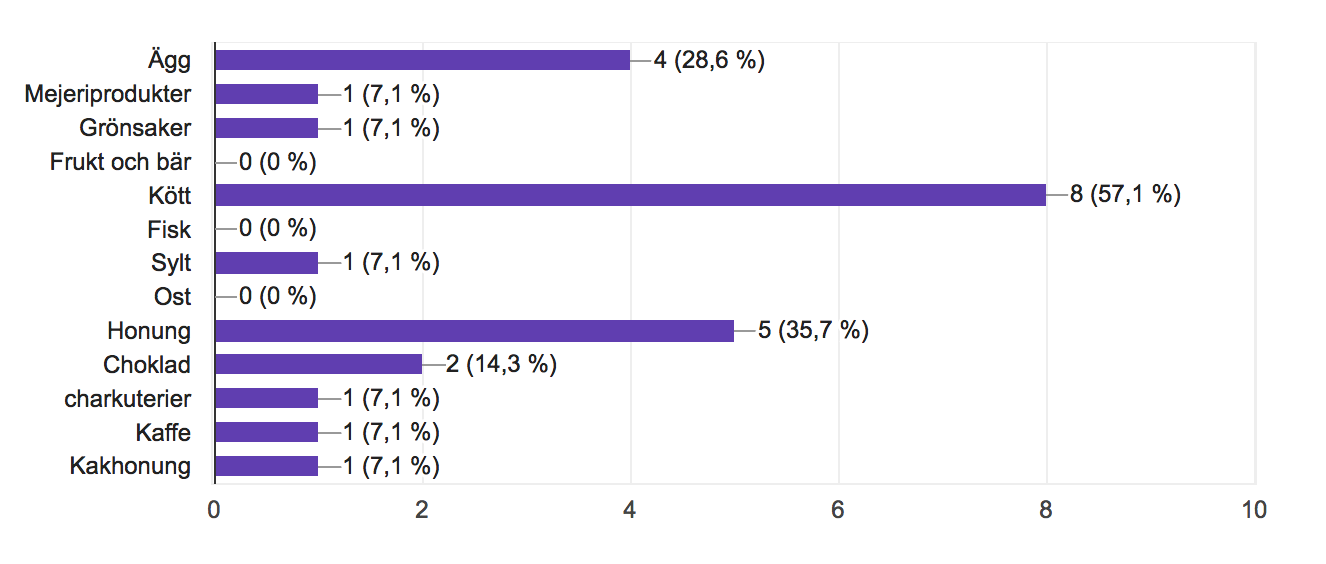
\includegraphics[scale=0.6]{1.png}
	\caption{Vad s\"aljer du f\"or typ av produkter?}
\end{figure}

\begin{figure}
	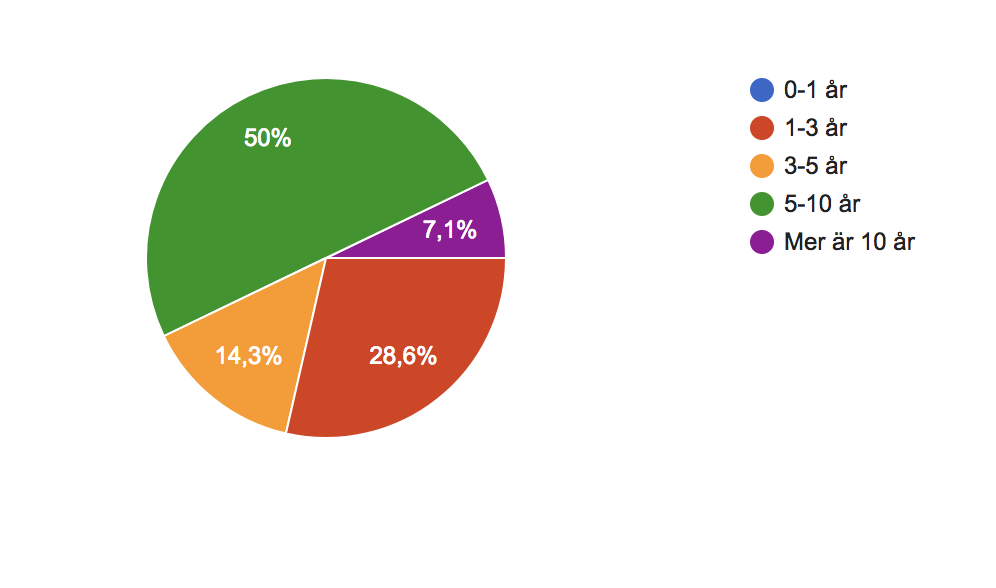
\includegraphics[scale=0.6]{2.png}
	\caption{Hur l\"ange har du s\'alt dessa varor?}
\end{figure}

\begin{figure}
	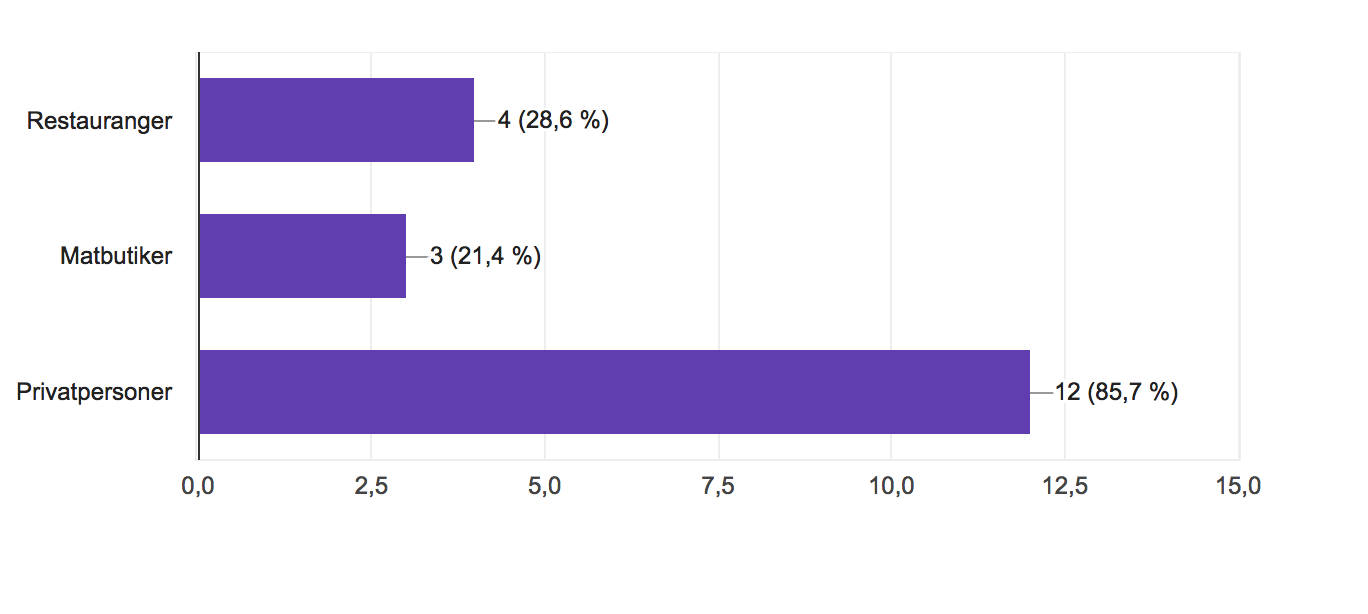
\includegraphics[scale=0.6]{3.png}
	\caption{Vad \"ar din huvudsakliga kundkrets?}
\end{figure}

\begin{figure}
	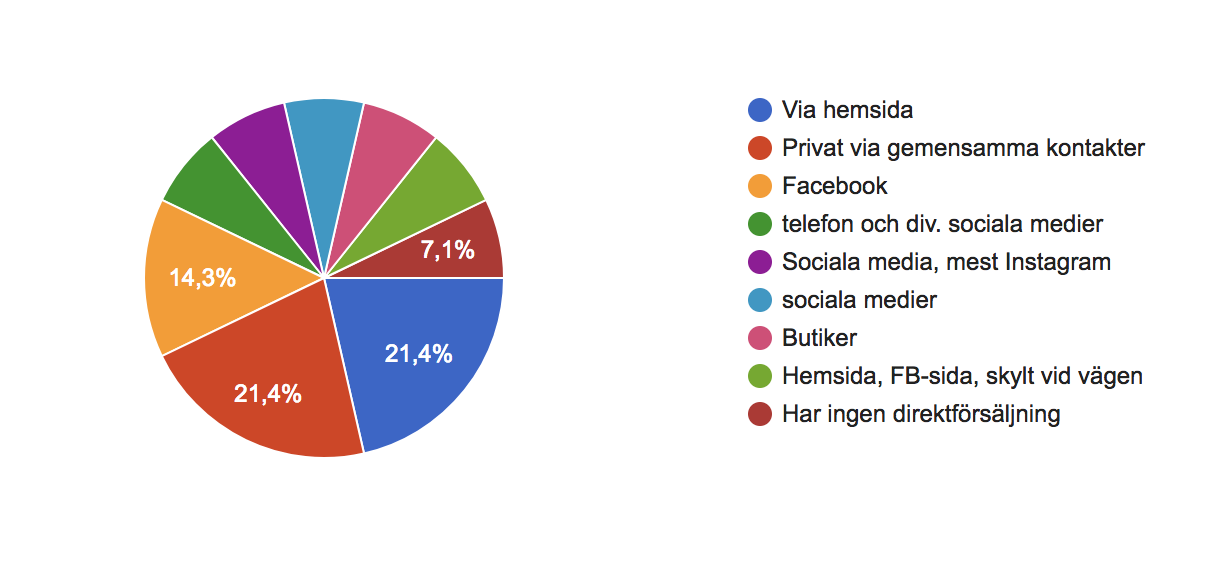
\includegraphics[scale=0.6]{4.png}
	\caption{P\'a vilket s\"att kommer kunder i kontakt med dig idag?}
\end{figure}

\begin{figure}
	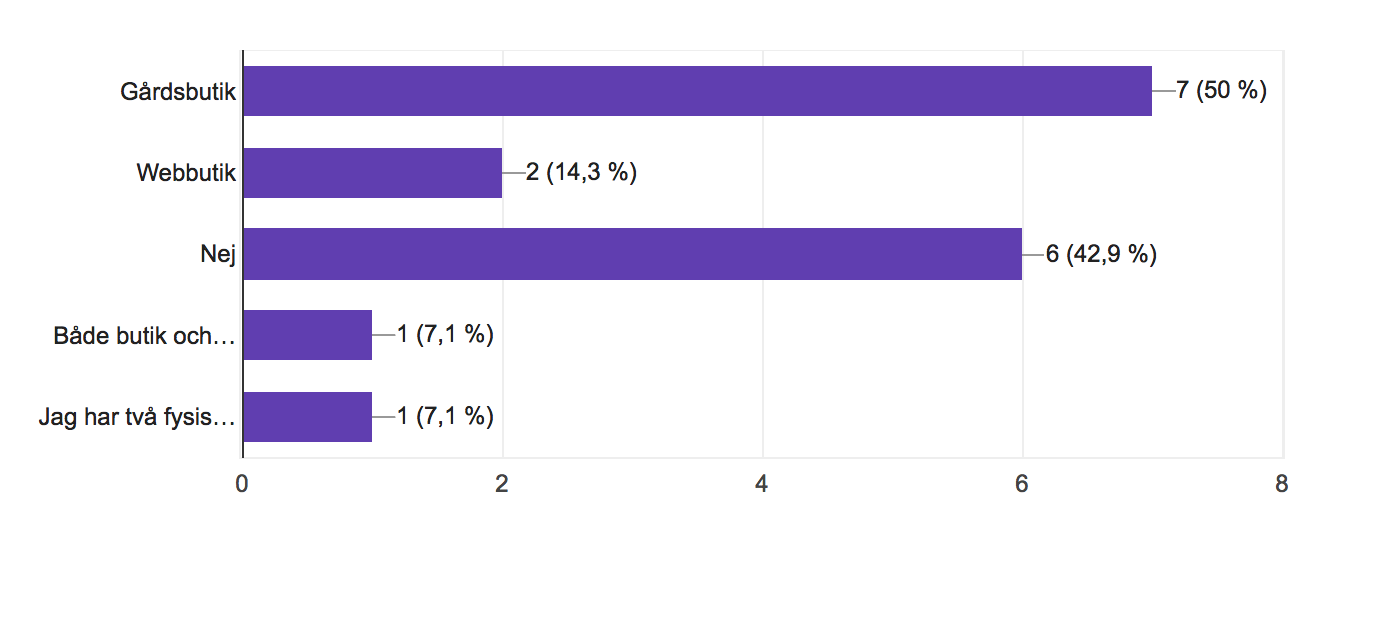
\includegraphics[scale=0.6]{5.png}
	\caption{Har du i dagsl\"aget en g\'ardsbutik eller webbutik?}
\end{figure}

\begin{figure}
	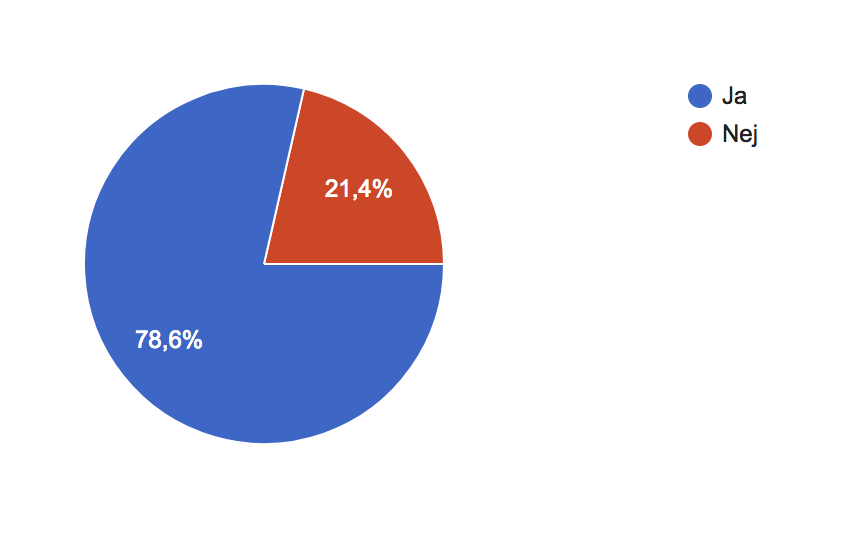
\includegraphics[scale=0.6]{6.png}
	\caption{Skulle du vara intresserad av att n\'a ut till fler privatpersoner?}
\end{figure}

\begin{figure}
	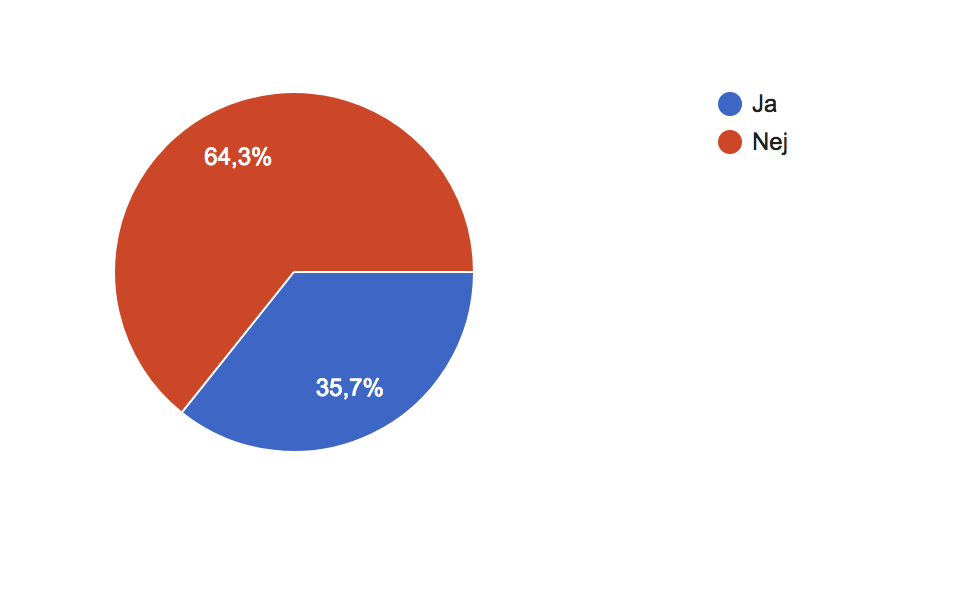
\includegraphics[scale=0.6]{7.png}
	\caption{Tror du att majoriteten av m\"ojliga kunder k\"anner till dig och vad du s\"aljer när de ska k\"opa varor som du kan leverera?}
\end{figure}

\begin{figure}
	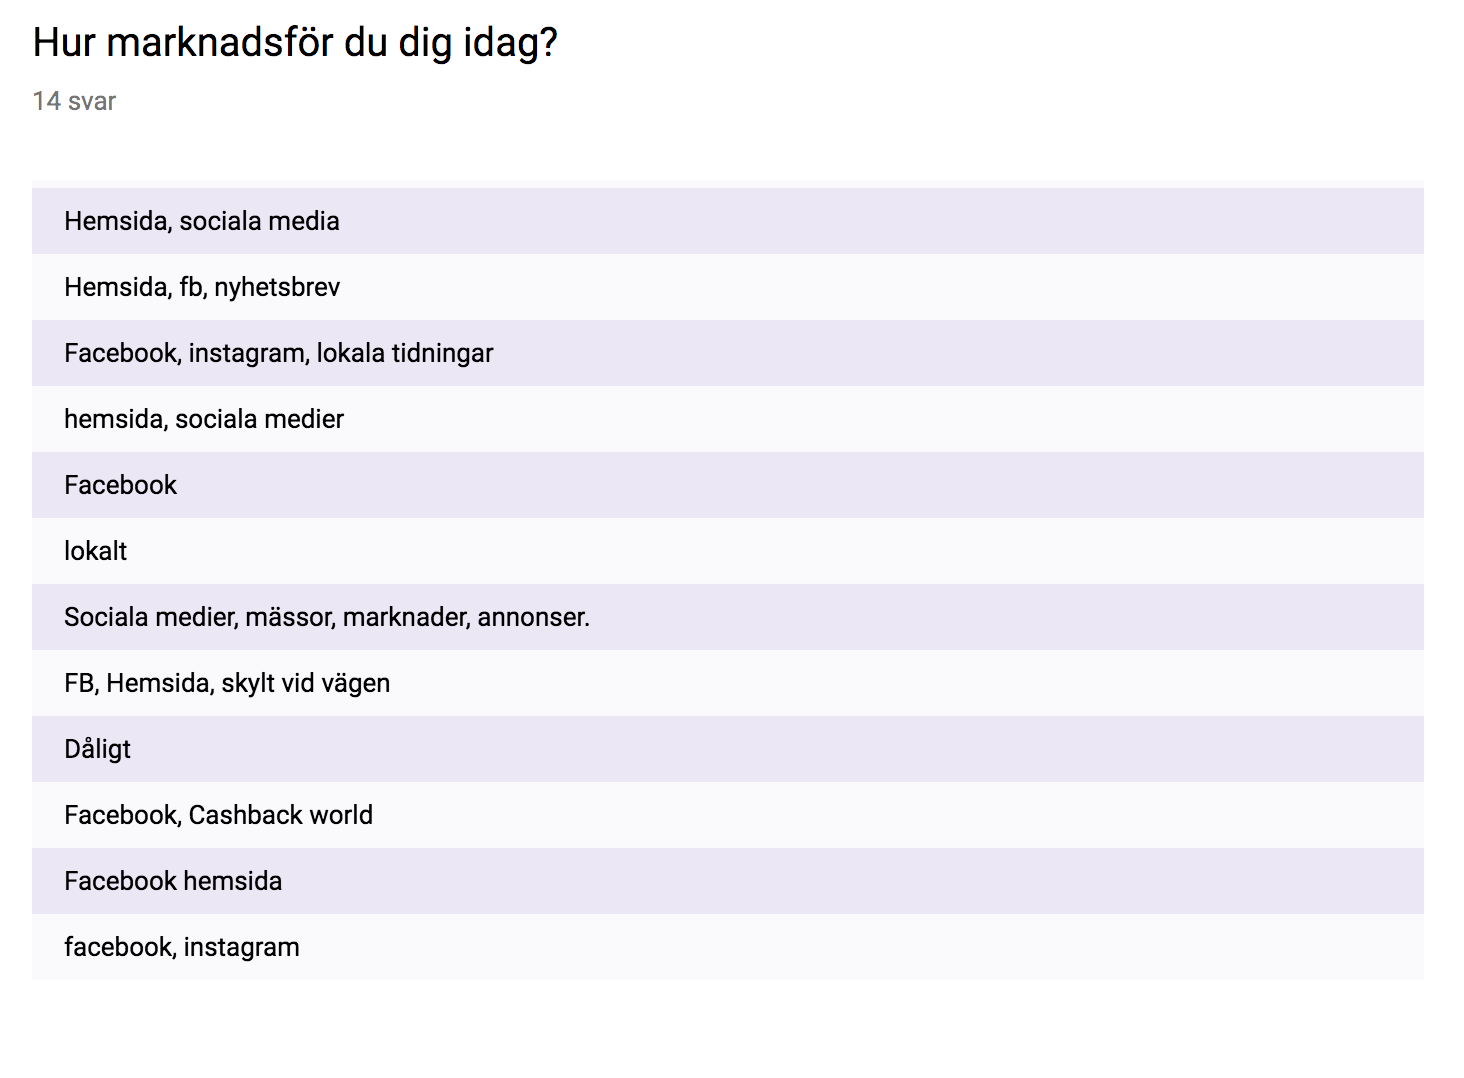
\includegraphics[scale=0.6]{8.png}
	\caption{Hur marknadsf\"or du dig idag?}
\end{figure}

\begin{figure}
	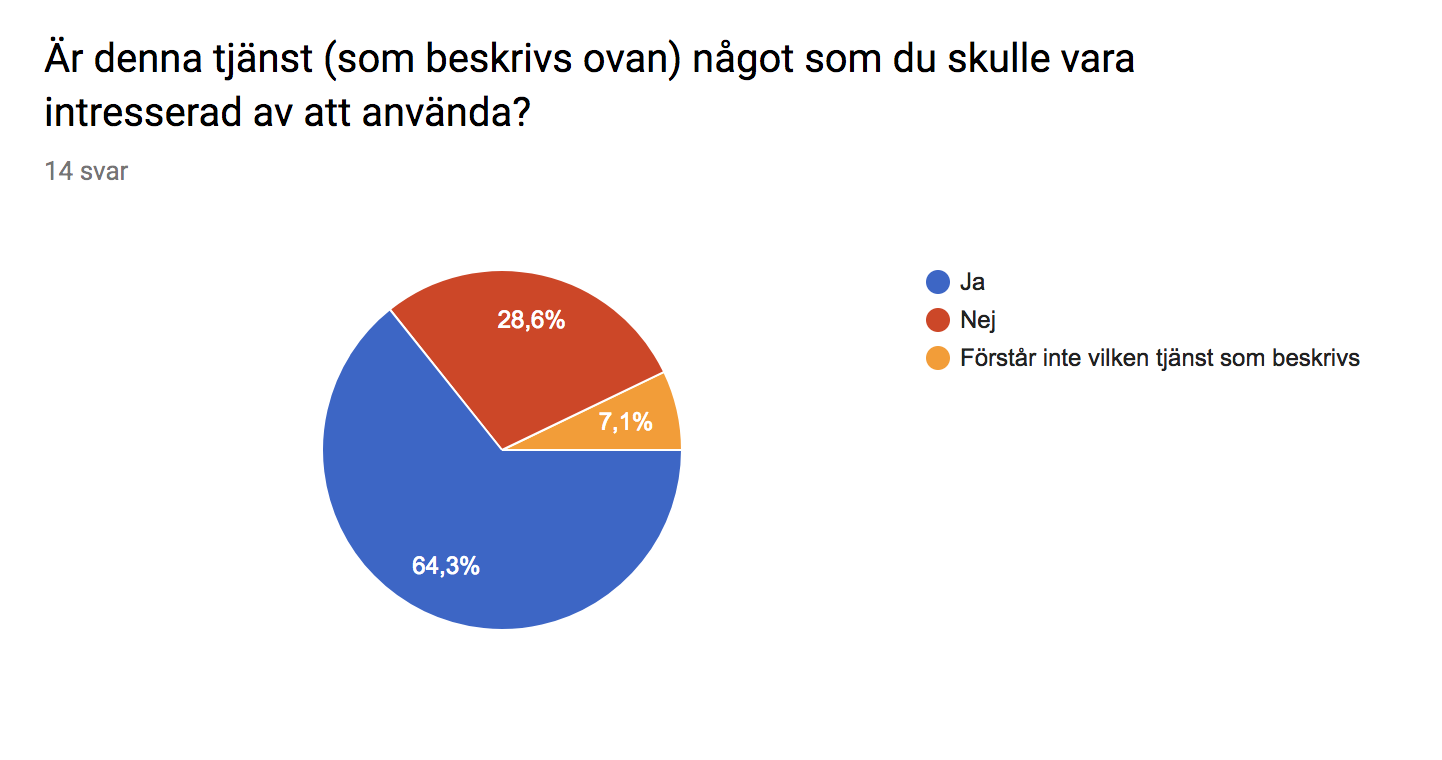
\includegraphics[scale=0.6]{9.png}
	\caption{\"Ar denna tj\"anst n\'agot som du skulle vara intresserad av att anv\"anda?}
\end{figure}

\begin{figure}
	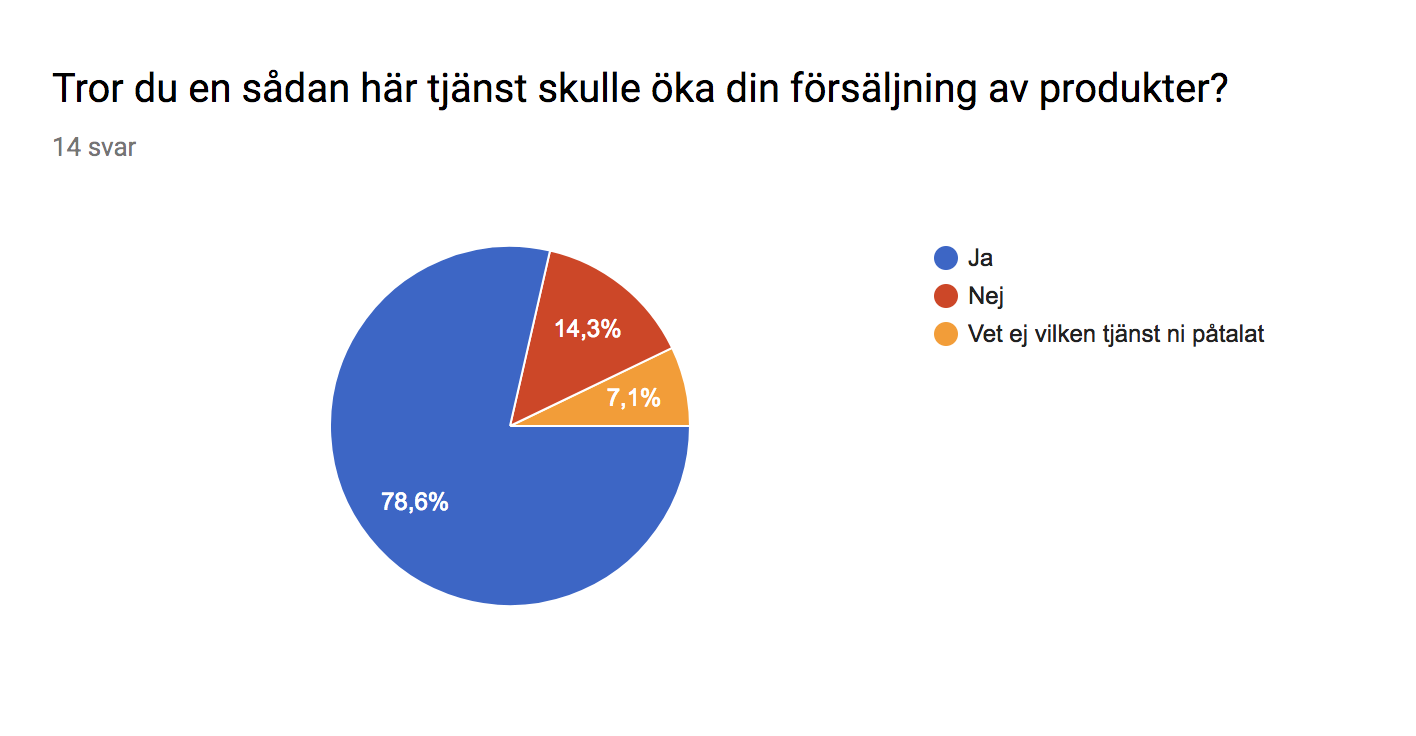
\includegraphics[scale=0.6]{10.png}
	\caption{Tror du att en s\'adan h\"ar tj\"anst skulle \"oka din f\"olrs\"aljning av produkter?}
\end{figure}

\begin{figure}
	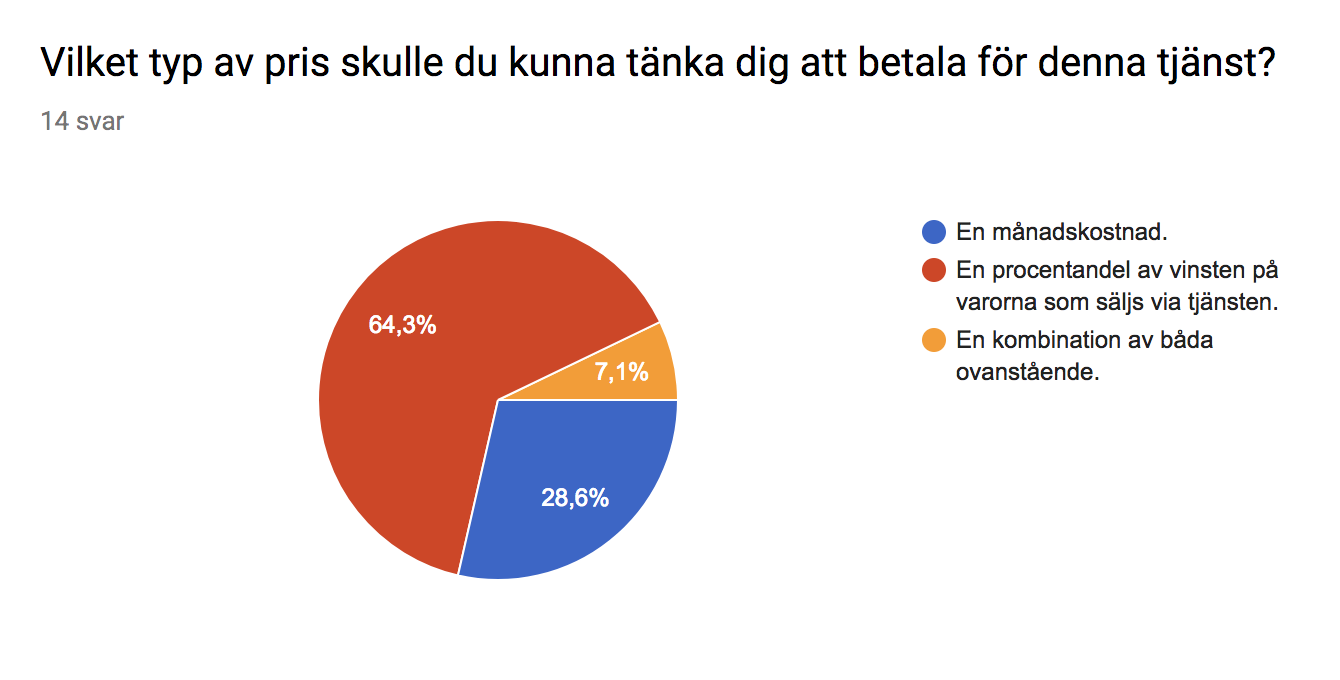
\includegraphics[scale=0.6]{11.png}
	\caption{Vilken typ av pris skulle du kunna t\"anka dig att betala för denna tj\"anst?}
\end{figure}

\begin{figure}
	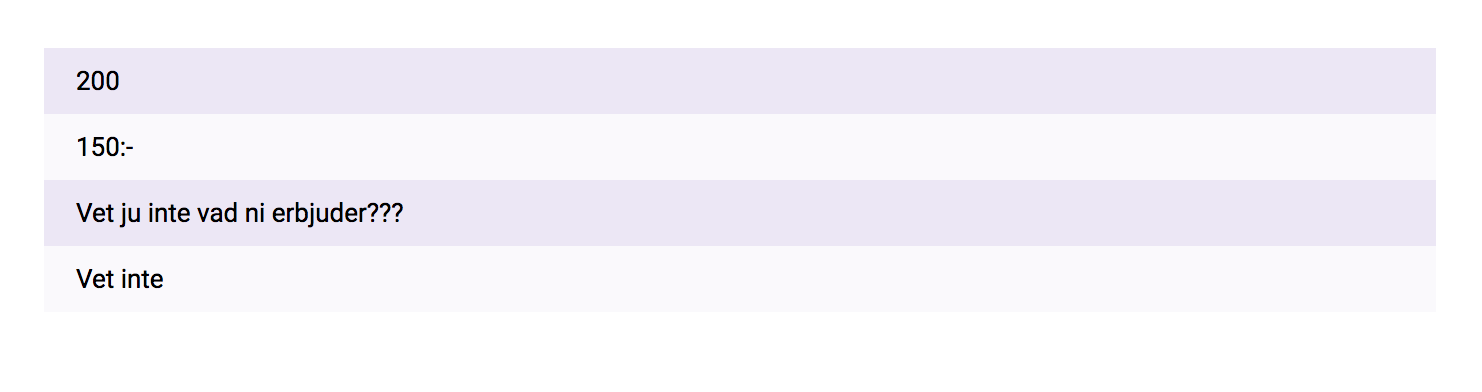
\includegraphics[scale=0.6]{12.png}
	\caption{Om en m\'anadskostnad, hur mycket?}
\end{figure}

\begin{figure}
	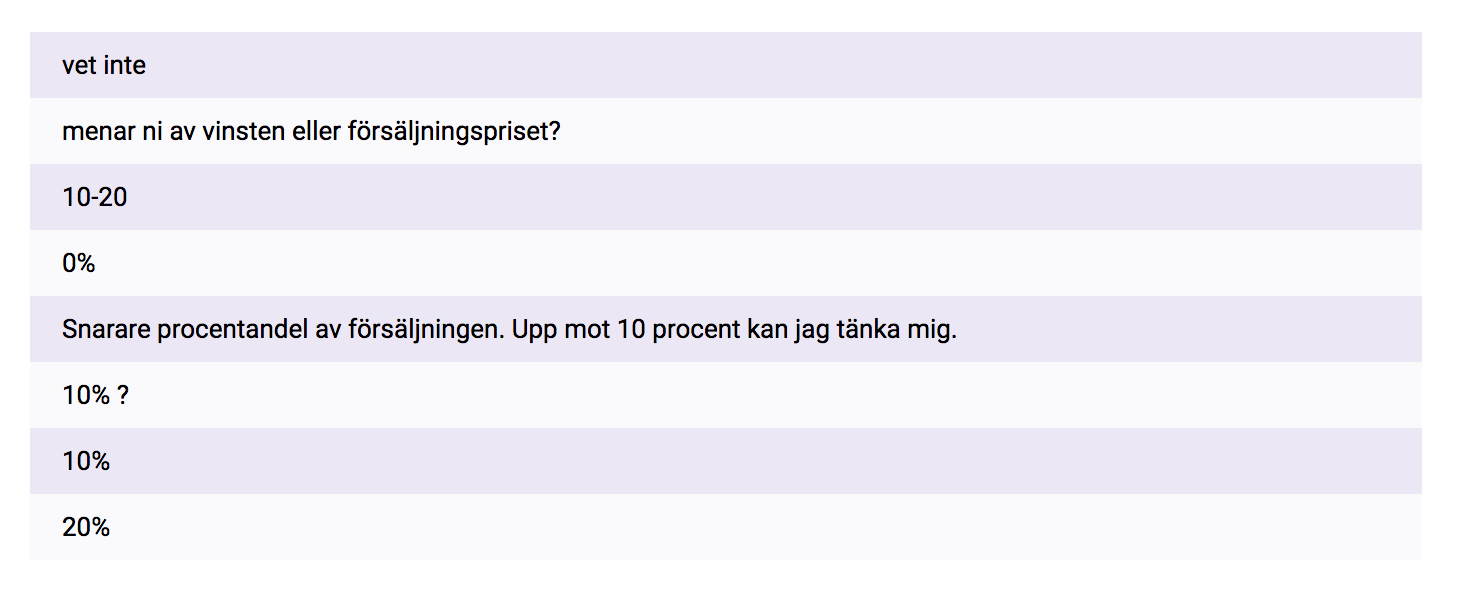
\includegraphics[scale=0.6]{13.png}
	\caption{Om en procentandel, hur mycket?}
\end{figure}

\begin{figure}
	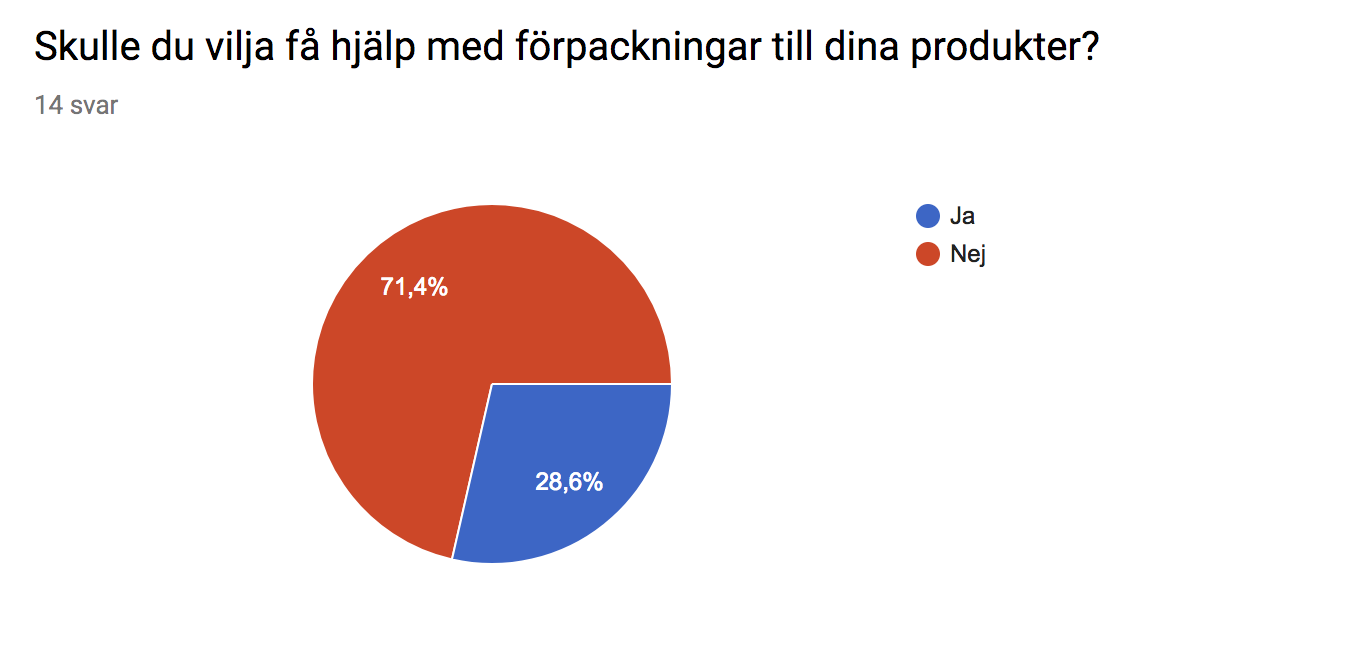
\includegraphics[scale=0.6]{14.png}
	\caption{Skulle du vilja f\'a hj\"alp med f\"orpackningar till dina produkter?}
\end{figure}


\begin{table}[tb]
\centering
\begin{tabular}{ | p{3cm} | p{2cm} | p{2cm} | p{2cm} | p{2cm} |}
 \hline
  & Antal & Eng\'angsutgifter & \'Arliga utgifter & \'Arliga inkomster\\ \hline
L\"oner (inklusive semesterl\"on, arbetsgivaravgift, f\"ors\"akring) & 3 &  & 324460 kr/pers &  \\ \hline
Programvaror (Creative Cloud) &1 &  & 7188 kr/pers &  \\ \hline
Macbook pro  & 3 & 18790 kr/st &  &  \\ \hline
F\"orvaringslokal, el och bredband &  &  & Hyra: 200000 kr, El: 2400 kr, Bredband: 4800 kr & \\ \hline
Kylsk\'ap  & 6 & 3000 kr/st &  & \\ \hline
Inredning & 3 skrivbord, 3 kontorsstolar & skrivbord: 400 kr/st, kontorsstolar 200 kr/st &  & \\ \hline
Eldrivenlastbil & 1 & 175000 kr/st &  & \\ \hline
Kamera & 1 & 3000 kr/st &  & \\ \hline
Marknadsf\"oring &  &  & Facebook: 3600 kr & \\ \hline
Server och Hemsida &  &  & 2988 kr & \\ \hline
Dom\"an &  &  & 119 kr & \\ \hline
Utveckling av hemsida &  & 10000 kr &  & \\ \hline
M\'anadskostnad medlemskap  &  &  &  & 1188 kr/st\\ \hline
Procentandel av f\"ors\"aljning  &  &  &  & 10 procent av vinsten\\ \hline
Fraktkostnader &  &  & T\"acks av kunden & \\ \hline
Totalt &  & 249370 & 1190525 & \\ \hline
Oms\"attning
scenario 1 &  &  kr &  & 11905250 kr\\ \hline
Bruttovinst scenario 1 &  &  &  & 0 kr\\ \hline
Oms\"attning scenario 2 &  &  &  & 24047520 kr\\ \hline
Bruttovinst
scenario 2 &  &  &  & 1256995 kr\\ \hline
Oms\"attning scenario 3 &  &  &  & 611880 kr\\ \hline
Bruttovinst scenario 3 &  &  &  & -1118645 kr\\ \hline

\end{tabular}
\caption{\label{tab:one} Ekonomisk budget}
\end{table}

\end{document}